\documentclass[]{article}
\usepackage{lmodern}
\usepackage{amssymb,amsmath}
\usepackage{ifxetex,ifluatex}
\usepackage{fixltx2e} % provides \textsubscript
\ifnum 0\ifxetex 1\fi\ifluatex 1\fi=0 % if pdftex
  \usepackage[T1]{fontenc}
  \usepackage[utf8]{inputenc}
\else % if luatex or xelatex
  \ifxetex
    \usepackage{mathspec}
  \else
    \usepackage{fontspec}
  \fi
  \defaultfontfeatures{Ligatures=TeX,Scale=MatchLowercase}
\fi
% use upquote if available, for straight quotes in verbatim environments
\IfFileExists{upquote.sty}{\usepackage{upquote}}{}
% use microtype if available
\IfFileExists{microtype.sty}{%
\usepackage{microtype}
\UseMicrotypeSet[protrusion]{basicmath} % disable protrusion for tt fonts
}{}
\usepackage[margin=1in]{geometry}
\usepackage{hyperref}
\hypersetup{unicode=true,
            pdftitle={Tourism Data Analysis},
            pdfborder={0 0 0},
            breaklinks=true}
\urlstyle{same}  % don't use monospace font for urls
\usepackage{color}
\usepackage{fancyvrb}
\newcommand{\VerbBar}{|}
\newcommand{\VERB}{\Verb[commandchars=\\\{\}]}
\DefineVerbatimEnvironment{Highlighting}{Verbatim}{commandchars=\\\{\}}
% Add ',fontsize=\small' for more characters per line
\usepackage{framed}
\definecolor{shadecolor}{RGB}{248,248,248}
\newenvironment{Shaded}{\begin{snugshade}}{\end{snugshade}}
\newcommand{\KeywordTok}[1]{\textcolor[rgb]{0.13,0.29,0.53}{\textbf{#1}}}
\newcommand{\DataTypeTok}[1]{\textcolor[rgb]{0.13,0.29,0.53}{#1}}
\newcommand{\DecValTok}[1]{\textcolor[rgb]{0.00,0.00,0.81}{#1}}
\newcommand{\BaseNTok}[1]{\textcolor[rgb]{0.00,0.00,0.81}{#1}}
\newcommand{\FloatTok}[1]{\textcolor[rgb]{0.00,0.00,0.81}{#1}}
\newcommand{\ConstantTok}[1]{\textcolor[rgb]{0.00,0.00,0.00}{#1}}
\newcommand{\CharTok}[1]{\textcolor[rgb]{0.31,0.60,0.02}{#1}}
\newcommand{\SpecialCharTok}[1]{\textcolor[rgb]{0.00,0.00,0.00}{#1}}
\newcommand{\StringTok}[1]{\textcolor[rgb]{0.31,0.60,0.02}{#1}}
\newcommand{\VerbatimStringTok}[1]{\textcolor[rgb]{0.31,0.60,0.02}{#1}}
\newcommand{\SpecialStringTok}[1]{\textcolor[rgb]{0.31,0.60,0.02}{#1}}
\newcommand{\ImportTok}[1]{#1}
\newcommand{\CommentTok}[1]{\textcolor[rgb]{0.56,0.35,0.01}{\textit{#1}}}
\newcommand{\DocumentationTok}[1]{\textcolor[rgb]{0.56,0.35,0.01}{\textbf{\textit{#1}}}}
\newcommand{\AnnotationTok}[1]{\textcolor[rgb]{0.56,0.35,0.01}{\textbf{\textit{#1}}}}
\newcommand{\CommentVarTok}[1]{\textcolor[rgb]{0.56,0.35,0.01}{\textbf{\textit{#1}}}}
\newcommand{\OtherTok}[1]{\textcolor[rgb]{0.56,0.35,0.01}{#1}}
\newcommand{\FunctionTok}[1]{\textcolor[rgb]{0.00,0.00,0.00}{#1}}
\newcommand{\VariableTok}[1]{\textcolor[rgb]{0.00,0.00,0.00}{#1}}
\newcommand{\ControlFlowTok}[1]{\textcolor[rgb]{0.13,0.29,0.53}{\textbf{#1}}}
\newcommand{\OperatorTok}[1]{\textcolor[rgb]{0.81,0.36,0.00}{\textbf{#1}}}
\newcommand{\BuiltInTok}[1]{#1}
\newcommand{\ExtensionTok}[1]{#1}
\newcommand{\PreprocessorTok}[1]{\textcolor[rgb]{0.56,0.35,0.01}{\textit{#1}}}
\newcommand{\AttributeTok}[1]{\textcolor[rgb]{0.77,0.63,0.00}{#1}}
\newcommand{\RegionMarkerTok}[1]{#1}
\newcommand{\InformationTok}[1]{\textcolor[rgb]{0.56,0.35,0.01}{\textbf{\textit{#1}}}}
\newcommand{\WarningTok}[1]{\textcolor[rgb]{0.56,0.35,0.01}{\textbf{\textit{#1}}}}
\newcommand{\AlertTok}[1]{\textcolor[rgb]{0.94,0.16,0.16}{#1}}
\newcommand{\ErrorTok}[1]{\textcolor[rgb]{0.64,0.00,0.00}{\textbf{#1}}}
\newcommand{\NormalTok}[1]{#1}
\usepackage{graphicx,grffile}
\makeatletter
\def\maxwidth{\ifdim\Gin@nat@width>\linewidth\linewidth\else\Gin@nat@width\fi}
\def\maxheight{\ifdim\Gin@nat@height>\textheight\textheight\else\Gin@nat@height\fi}
\makeatother
% Scale images if necessary, so that they will not overflow the page
% margins by default, and it is still possible to overwrite the defaults
% using explicit options in \includegraphics[width, height, ...]{}
\setkeys{Gin}{width=\maxwidth,height=\maxheight,keepaspectratio}
\IfFileExists{parskip.sty}{%
\usepackage{parskip}
}{% else
\setlength{\parindent}{0pt}
\setlength{\parskip}{6pt plus 2pt minus 1pt}
}
\setlength{\emergencystretch}{3em}  % prevent overfull lines
\providecommand{\tightlist}{%
  \setlength{\itemsep}{0pt}\setlength{\parskip}{0pt}}
\setcounter{secnumdepth}{0}
% Redefines (sub)paragraphs to behave more like sections
\ifx\paragraph\undefined\else
\let\oldparagraph\paragraph
\renewcommand{\paragraph}[1]{\oldparagraph{#1}\mbox{}}
\fi
\ifx\subparagraph\undefined\else
\let\oldsubparagraph\subparagraph
\renewcommand{\subparagraph}[1]{\oldsubparagraph{#1}\mbox{}}
\fi

%%% Use protect on footnotes to avoid problems with footnotes in titles
\let\rmarkdownfootnote\footnote%
\def\footnote{\protect\rmarkdownfootnote}

%%% Change title format to be more compact
\usepackage{titling}

% Create subtitle command for use in maketitle
\providecommand{\subtitle}[1]{
  \posttitle{
    \begin{center}\large#1\end{center}
    }
}

\setlength{\droptitle}{-2em}

  \title{Tourism Data Analysis}
    \pretitle{\vspace{\droptitle}\centering\huge}
  \posttitle{\par}
    \author{}
    \preauthor{}\postauthor{}
      \predate{\centering\large\emph}
  \postdate{\par}
    \date{31 July 2019}

\usepackage{booktabs}
\usepackage{longtable}
\usepackage{array}
\usepackage{multirow}
\usepackage{wrapfig}
\usepackage{float}
\usepackage{colortbl}
\usepackage{pdflscape}
\usepackage{tabu}
\usepackage{threeparttable}
\usepackage{threeparttablex}
\usepackage[normalem]{ulem}
\usepackage{makecell}
\usepackage{xcolor}

\begin{document}
\maketitle

\section{BoxCox Transformation}\label{boxcox-transformation}

\begin{tabular}{l|r|r|r}
\hline
R.method & Bias & Unbiased (Method 1) & Unbiased (Method 2)\\
\hline
Base & 4.64 & 3521.02 & 6.73\\
\hline
Bottom-up & 6.47 & 5.29 & 8.10\\
\hline
MinT(Shrink) & 4.35 & 4.23 & 4.67\\
\hline
OLS & 4.50 & 2938.01 & 6.38\\
\hline
WLS & 4.90 & 4.40 & 5.55\\
\hline
\end{tabular}

\section{More analysis on BoxCox transformed
results}\label{more-analysis-on-boxcox-transformed-results}

\begin{verbatim}
## # A tibble: 1 x 4
##   Series  Bias Unbiased_M1 `Bias-Unbiase`
##   <fct>  <dbl>       <dbl>          <dbl>
## 1 Total   275.     386984.       -386710.
\end{verbatim}

Bias correction is giving wiered results for \texttt{Total} series.

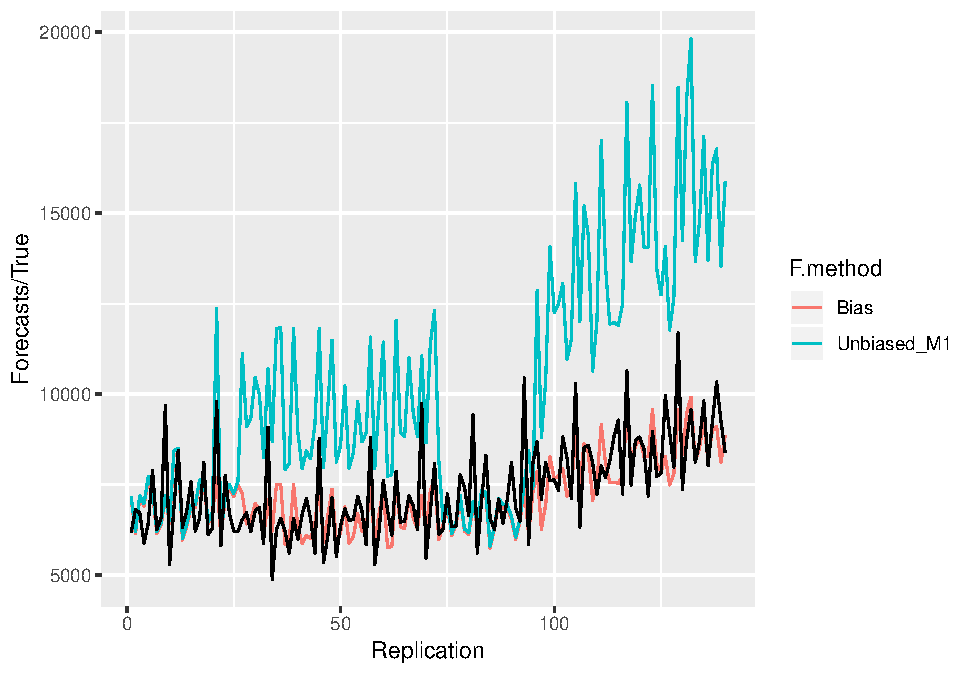
\includegraphics{TourismData-Final-results_files/figure-latex/unnamed-chunk-3-1.pdf}

\begin{Shaded}
\begin{Highlighting}[]
\NormalTok{DF_BoxCoxTrans_Tot_h1 }\OperatorTok\StringTok{ }
\StringTok{  }\KeywordTok{spread}\NormalTok{(}\DataTypeTok{key =} \StringTok{`}\DataTypeTok{Forecasts/Actual}\StringTok{`}\NormalTok{, }\DataTypeTok{value =}\NormalTok{ Val) }\OperatorTok\StringTok{ }
\StringTok{  }\KeywordTok{mutate}\NormalTok{(}\StringTok{"Unb-Act"}\NormalTok{ =}\StringTok{ }\NormalTok{Unbiased_M1 }\OperatorTok{-}\StringTok{ }\NormalTok{Actual) }\OperatorTok\StringTok{ }
\StringTok{  }\KeywordTok{filter}\NormalTok{(}\StringTok{`}\DataTypeTok{Unb-Act}\StringTok{`}\OperatorTok{>}\DecValTok{1000}\NormalTok{)}
\end{Highlighting}
\end{Shaded}

\begin{verbatim}
##    Replication    Actual     Bias Unbiased_M1   Unb-Act
## 1           24  6690.320 7942.644    7929.872  1239.551
## 2           67  6922.011 6256.862   32427.930 25505.920
## 3           68  6253.403 5990.885   28965.728 22712.325
## 4           69  9742.298 9074.247   88888.278 79145.980
## 5           71  6735.583 6492.927   35741.613 29006.030
## 6           73  6129.598 6408.122   40797.225 34667.627
## 7           74  6266.592 6297.023   32998.078 26731.487
## 8           75  7240.105 7236.467   47696.759 40456.654
## 9           76  6333.832 6456.888   35207.147 28873.315
## 10          77  6347.804 6727.321   39234.151 32886.347
## 11          78  7770.601 7162.167   46393.968 38623.367
## 12          79  7427.809 6689.464   38641.113 31213.304
## 13          80  6640.508 6034.327   29470.252 22829.744
## 14          81  9419.311 9672.074  106057.019 96637.708
## 15          82  5605.903 5534.823   23602.321 17996.418
## 16          83  7058.426 6578.873   36903.003 29844.577
## 17          85  6566.996 6308.722   33039.816 26472.820
## 18          86  6258.781 6578.185    8721.849  2463.068
## 19          87  7098.180 6994.092   43522.680 36424.500
## 20          88  6436.991 6633.680   37729.921 31292.930
## 21          89  7071.804 6554.580   36555.710 29483.905
## 22          90  8106.166 7703.135   12245.860  4139.695
## 23          91  6839.574 7390.927   50397.661 43558.087
## 24          92  6482.379 6460.287   35188.677 28706.298
## 25          93 10445.812 9631.840  104815.092 94369.280
## 26          94  5847.470 5615.639   24482.840 18635.370
## 27          95  8089.742 7008.365   51987.132 43897.390
## 28          96  8678.255 8423.320   86514.330 77836.075
## 29          97  7095.224 6789.855   47695.463 40600.240
## 30          98  8116.618 6635.950   44825.584 36708.966
## 31          99  7611.168 7986.305   11211.788  3600.620
\end{verbatim}

Very large bias corrected forecasts are given for some replications. For
example in the rolling window Jul-2003 to Oct-2011. Observing the model
auto.arima fits:

\begin{verbatim}
## Warning: Missing column names filled in: 'X1' [1]
\end{verbatim}

\begin{verbatim}
## Parsed with column specification:
## cols(
##   .default = col_double(),
##   `Month returned from trip` = col_character()
## )
\end{verbatim}

\begin{verbatim}
## See spec(...) for full column specifications.
\end{verbatim}

\begin{verbatim}
## Series: TS 
## ARIMA(0,0,0)(2,1,1)[12] with drift 
## Box Cox transformation: lambda= -0.9999242 
## 
## Coefficients:
\end{verbatim}

\begin{verbatim}
## Warning in sqrt(diag(x$var.coef)): NaNs produced
\end{verbatim}

\begin{verbatim}
##          sar1     sar2     sma1  drift
##       -0.1604  -0.3213  -0.7427      0
## s.e.   0.0666   0.0815   0.1256    NaN
## 
## sigma^2 estimated as 1.429e-07:  log likelihood=878.67
## AIC=-1747.34   AICc=-1746.61   BIC=-1734.95
## 
## Training set error measures:
##                    ME     RMSE      MAE      MPE     MAPE     MASE
## Training set 758.0031 2294.668 1101.829 9.975516 15.40116 2.203493
##                   ACF1
## Training set 0.8644324
\end{verbatim}

The estimated drift term has a very large standard error. Further the
variance of \(\hat{y}_{t+1}\) is 6903171.42872441 which is very large

\section{Log Transformation}\label{log-transformation}

\begin{tabular}{l|r|r|r}
\hline
R.method & Bias & Unbiased (Method 1) & Unbiased (Method 2)\\
\hline
Base & 4.47 & 4.43 & 4.51\\
\hline
Bottom-up & 6.36 & 5.26 & 8.06\\
\hline
MinT(Shrink) & 4.32 & 4.16 & 4.61\\
\hline
OLS & 4.34 & 4.31 & 4.36\\
\hline
WLS & 4.82 & 4.38 & 5.43\\
\hline
\end{tabular}


\end{document}
